\documentclass[11pt]{article}
\usepackage{acl2015}
\usepackage{times}
\usepackage{hhline}
\usepackage{pbox}
\usepackage{latexsym}
\usepackage{amsmath}
\usepackage{multirow}
\usepackage{url}
\usepackage{setspace}
\usepackage{array}
\usepackage{graphicx}
\newcommand{\chprob}[2]{\mathbf{#1} \mid \mathbf{#2}}
\newcommand{\word}[1]{\mathbf{#1}}
%\linespread{2}

%\doublespacing

\DeclareMathOperator*{\argmax}{arg\,max}
\setlength\titlebox{6.5cm}    % Expanding the titlebox

\title{Decipherment with Word Embeddings through Multinomial Regression}

%\author{Qing Dou, Ashish Vaswani, Kevin Knight, and Chris Dyer \\
%  Information Sciences Institute \\Department of Computer Science\\
%  University of Southern California \\
%  {\tt \{qdou,knight\}@isi.edu} \\}  

\date{}

\begin{document}
\maketitle
\begin{abstract}
We introduce a base distribution derived from word embeddings similarities into Bayesian decipherment. Learning of embeddings similarities are combined with decipherment in a stochastic EM process. Experiment results show that the base distribution is highly beneficial to decipherment, improving the state-of-the-art decipherment accuracy from 26.0\% to 59.1\% for Spanish and English, 5.1\% to 11.2\% for Malagasy and English. 
\end{abstract}

\section{Introduction}
Tremendous advance in Machine Translation(MT) has been made since we apply machine learning techniques to learn translation rules automatically from parallel data. However, the reliance on parallel data also limits development and application of high quality MT systems as the amount of parallel data is far from adequate for low density languages and various domains.

In general, it is easier to obtain comparable monolingual data. The ability to learn translations from monolingual data could alleviate obstacles caused by insufficient parallel data. Motivated by this idea, researchers have proposed different approaches to tackle this problem. 

The approaches to find translations from monolingual data can be largely divided into two groups. The first group is based on the idea proposed by \newcite{Rapp:1995}, where words are represented as context vectors, and two words are likely to be translations if their context vectors are similar. Initially, the vectors contain just context words. Later, a number of work has extended this approach by introducing more features\cite{haghighi-EtAl:2008:ACLMain,Garera:2009,Bergsma:2011,Daume:2011:DAM:2002736.2002819,irvine-callisonburch:2013,irvine-callisonburch:2013:WMT}, and using more abstract representation such as word embeddings\cite{KlementievCOLING}.

Another interesting approach to solve this problem is through decipherment. It has drawn significant amount of interests in the past few years\cite{ravi-knight:2011,Nuhn:2012,dou-knight:2013:EMNLP,ravi:2013}, and has been shown to improve machine translations. Decipherment views foreign languages as ciphers for English, and finds a translation table that converts foreign texts into sensible English. 

Both approaches have been shown to improve quality of MT systems for domain adaptation \cite{Daume:2011:DAM:2002736.2002819,Dou:2012,irvineQuirkDaumeEMNLP13} and low density languages \cite{irvine-callisonburch:2013:WMT,dou-vaswani-knight:2014:EMNLP2014}. Meanwhile, they also have their own advantages and disadvantages. While the former can take larger context into account, it requires high quality seed lexicons to learn a mapping between two vector spaces. In contrast, the latter does not depend on any seed lexicon, but is only able to look at limited context informed by either a bigram or trigram language model.  

In this work, we take advantages of both approaches and combine them in a joint inference process. More specifically, we extend previous work in large scale Bayesian decipherment by introducing a better base distribution, which is derived from similarities of word embedding vectors. The main contributions of this work are:

\begin{itemize}
\item We propose a new framework that combines two previous approaches that find translations from monolingual data.

\item We show the new approach improves the state-of-the art decipherment accuracy by over two folds for different language pairs(Spanish-English, Malagasy-English). 

\item We make our program a standard toolkit for finding translations from monolingual data for future research.
\end{itemize}
\section{Decipherment Model}
In this section, we describe the decipherment model, upon which this work is built on. We first briefly introduce recent advances made in decipherment work, then describe the state-of-the-art approach, and in the end, bring up the problem that we address in this work. 

Unsupervised learning of translations from non-parallel is an old and challenging problem. In recent years, there has been growing interests in approaching it using decipherment techniques. \newcite{ravi-knight:2011} built an MT system using only non parallel data for translating movie subtitles. \newcite{Dou:2012} and \newcite{Nuhn:2012} made decipherment scalable to handle larger vocabulary. \newcite{dou-knight:2013:EMNLP} improved decipherment accuracy significantly by using dependency information between words. 

Throughout this paper, we use $f$ to denote target language or ciphertext tokens, and $e$ to denote source language or plaintext tokens. Given ciphertext $\mathbf{\cipher}:f_{1}...f_{n}$, the task of decipherment is to find a set of parameters $P(f_{i}|e_{i})$ that convert $F$ to sensible plaintext. The ciphertext $F$ can either be full sentences \cite{ravi-knight:2011,Nuhn:2012} or simply bigrams \cite{dou-knight:2013:EMNLP}. Since using bigrams and their counts significantly speeds up decipherment, in this work, we also see observed the data as bigrams, where $ \mathbf{\cipher} = \{ \mathbf{\cipher}^n \}_{n=1}^{N} = \{ \cipher_1^n,\cipher_2^n \}_{n=1}^{N} $. 

Motivated by the idea from \newcite{Weaver:1955}, we model a generate an observed bigram $\mathbf{\cipher}^n$ with the following generative story:

\begin{itemize}
\item  First, a languae model $P(\mathbf{\plain})$ generates a sequence of two plaintext tokens $e_{1}^n,e_{2}^n$ with probability $P(e_{1}^n,e_{2}^n)$.
\item  Then, substitute $\plain_{1}^n$ with $\cipher_{1}^n$ and $\plain_{2}^n$ with $\cipher_{2}^n$ with probability $P(\cipher_{1}^n \mid e_{1}^n) \cdot P(f_{2}^n \mid e_{2}^n)$.
\end{itemize}

Based on the above generative story, the probability of any cipher bigram $\mathbf{\cipher^n}$ is:
%
\[
\label{p_cipher}
P(\mathbf{\cipher}^n) =  \sum_{e_{1} e_{2}} P(e_{1}e_{2}) \prod_{i=1}^{2}P(f_{i}^n \mid e_{i})
\]
%

Let the entire ciphertext corpus contains $N$ such bigrams $F_{1}...F_{N}$, we write down the probability of the ciphertext corpus as:
%
\[
\label{p_corpus}
P( \{ \mathbf{\cipher}^n \}_{n=1}^{N} ) =  \prod_{n=1}^{N} P(\mathbf{\cipher}^{n})
\]
%

There are two sets of parameters in the model: the channel probabilities, \{ $P(\cipher \mid \plain) \} $, and the bigram language model probabilities $\{ P(\plain' \mid \plain) \} $, where $\cipher$ ranges over the ciphertext vocabulary and $\plain,\plain'$ range over the plaintext vocabulary. Given a plaintext bigram language model, the training objective is to learn $P(\cipher \mid \plain)$ that maximize $P( \{ \mathbf{\cipher}^n \}_{n=1}^{N} )$. When formulated like this, one can directly apply EM to solve the problem \cite{knight-EtAl:2006}. However, EM has time complexity $O( N\cdot V_{e}^{2})$ and space complexity $O(V_{f}\cdot V_{e})$, where $V_{f}$, $V_{e}$ are the sizes of ciphertext and plaintext vocabularies respectively, and $N$ is the number of cipher bigrams. This makes the EM approach unable to handle long ciphertext with large vocabulary size. 
%Unfortunately, EM is not scalable when $V_{f}$, $V_{e}$, and $N$ are very large.
%$\cipher \in 1,\ldots,V_{\plain}$ and $\plain, \plain' \in 1,\ldots,V_e$

An alternative approach to solve the problem is to apply Bayesian inference \cite{ravi-knight:2011,Dou:2012}. We assume that $P(\cipher \mid \plain)$ and $P(\plain' \mid \plain)$ are drawn from a Dirichet distribution with hyper-parameters $\alpha_{\cipher,\plain}$ and $\alpha_{\plain,\plain'}$, that is: 

\begin{align*}
P(\cipher \mid \plain) & \sim Dirichlet(\alpha_{\cipher,\plain}) \\ 
P(\plain \mid \plain') & \sim Dirichlet(\alpha_{\plain,\plain'}).
%P(C=0 \mid x) &= \frac{k q(x)}{\frac{n}Z p(x) + k q(x)} \\
%P(C=1 \mid x) &= \frac{\frac{n}Z p(x)}{\frac{n}Z p(x) + k q(x)}
\end{align*}

The remainder of the generative story is the same as the noisy channel model for decipherment. In the next section, we shall describe how we learn the hyper parameters of the Dirichlet prior. Given $\alpha_{\cipher,\plain}$ and $\alpha_{\plain,\plain'}$, The joint likelihood of the complete data and the parameters,
\begin{align} \label{joint_likelihood}
&P( \{ \mathbf{\cipher}^n , \mathbf{\plain}^n \}_{n=1}^{N}, \{ P(\cipher \mid \plain) \}, \{ P(\plain \mid \plain') \} )  \notag \\
 &= P( \{ \mathbf{\cipher}^n \mid \mathbf{\plain}^n \}_{n=1}^{N}, \{ P(\cipher \mid \plain) \}) \notag \\
     &P(  \{  \mathbf{\plain}^n \}_{n=1}^{N},P(\plain \mid \plain')) \notag \notag \\
 &= \prod_{\plain}  \frac{\dirgamma{\sum_{\cipher} \alpha_{\cipher,\plain}}} {\prod_{\cipher} \dirgamma{\alpha_{\plain,\cipher}}} \prod_{\cipher} P(\cipher \mid \plain)^{\#(\plain,\cipher)+\alpha_{\plain,\cipher} -1}  \notag \\
  &\prod_{\plain}  \frac{\dirgamma{\sum_{\plain'} \alpha_{\plain,\plain'}}} {\prod_{\plain'} \dirgamma{\alpha_{\plain,\plain'}}} \prod_{\cipher} P(\plain \mid \plain')^{\#(\plain,\plain')+\alpha_{\plain,\plain'} -1} , 
\end{align}

where $\#(\plain,\cipher)$ and $\#(\plain,\plain')$ are the counts of the translated word pairs and plaintext bigram pairs in the complete data, and $\dirgamma{\cdot}$ is the Gamma function. Unlike EM, in Bayeisan decipherment, we no longer search for parameters $P(\cipher \mid \plain)$ that maximize the likelihood of the observed ciphertext. Instead, we draw samples from posterior distribution of the plaintext sequences given the ciphertext. Under the above Bayesian decipherment model, we can show that the probability of a particular cipher word $\cipher_{j}$ having a value $k$, given the current plaintext word, and $\mathbf{\cipher}_{-j}$ and $\mathbf{\plain}_{-j}$, the samples for all the other plaintext and ciphertext words, 

\begin{equation} \label{prob_bayes_ciphertext}
P(\cipher_j = k \mid \plain_j,\mathbf{\cipher}_{-j}, \mathbf{\plain}_{-j}) = \frac{\#(k, \plain_j)_{-j} + \alpha_{\plain_j,k}}{\#(\plain_j)_{-j}+\sum_{\cipher} \alpha_{\plain_j,\cipher}}.
\end{equation}

Where, $\#(k, \plain_j)_{-j}$ and $\#(\plain_j)_{-j}$ are the counts of the ciphertext, plaintext word pair and plaintext word in the samples excluding $\cipher_j$ and $\plain_j$. Similarly, the probability of a plaintext word $\plain_j$ taking a value $l$ given samples for all other plaintext words, 
\begin{equation} \label{prob_bayes_plaintext}
P(\plain_j = l \mid \mathbf{\plain}_{-j}) = \frac{\#(l, \plain_{j-1})_{-j} + \alpha_{l,\plain_{j-1}}} {\#(\plain_{j-1})_{-j} + \sum_{\plain} \alpha_{\plain,\plain_{j-1}}}.
\end{equation}


%\begin{equation}
%\end{equation}

Since we have large amounts of plaintext data, we can train a high quality bigram language model, $P_{LM}(\plain \mid \plain')$ and use it to guide our samples and learn a better posterior distribution. For that, we define $\alpha_{\plain,\plain'} = \alpha P_{LM}(\plain \mid \plain')$, and set $\alpha$ to be very high. The probability of a plaintext word (Equation~\ref{prob_bayes_plaintext}) is now

\begin{equation} \label{prob_bayes_plaintext_lm}
P(\plain_j = l \mid \mathbf{\plain}_{-j}) \approx P_{LM}(l \mid \plain_{j-1}).
\end{equation}

\marginpar{We have to say that in previous work , $\alpha_{\plain,\cipher}$ has been set to $\alpha * uniform$}. To sample from the posterior, we iterate over the observed ciphertext bigram tokens and use equations~\ref{prob_bayes_ciphertext} and~\ref{prob_bayes_plaintext_lm} to sample a plaintext token with probability

\begin{align*}
P( \plain_j \mid \mathbf{\plain}_{-j}, \mathbf{\cipher} ) \propto & P_{LM}(\plain_j \mid \plain_{j-1}) \times \\
                                                                                                & P(\cipher_j \mid \plain_j,\mathbf{\cipher}_{-j}, \mathbf{\plain}_{-j}).
\end{align*}

\iffalse
%
\[
\label{p_sample}
P_{sample}(e_{1}e_{2}) =  P(e_{1}e_{2}) \prod_{i=1}^{2}P_{CRP}(f_{i}|e_{i})
\]
%
In the above equation, the translation probability $P_{CRP}(f_{i}|e_{i})$ is modeled by Chinese Restaurant Process(CRP), and is defined in Equation \ref{p_channel}.
%
\[
\label{p_channel}
P_{CRP}(f_{i}|e_{i}) = \frac{\alpha P_0(f_{i}|e_{i})+count(f_{i},e_{i})}{\alpha+count(e_{i})}
\]
%
where $P_{0}$ is a base distribution, also known as a prior, and $\alpha$ is a parameter that controls how much we trust the base distribution. $count(f_{i},e_{i})$ and $count(e_{i})$ record the number of times $f_{i},e_{i}$ and $e_{i}$ appear in previously generated samples respectively. The base distribution is given independently, and in all the previous work, it is set to uniform.
\fi

At the end of sampling, we compute $P(\cipher \mid \plain)$ from ciphertext and its plaintext samples using maximum likelihood estimation:

\[
\label{mlh_estimation}
P(\cipher \mid \plain) =  \frac{\#(\cipher,\plain)}{\#(\plain)}.
\]

In the next section, we will describe how we model and learn an appropriate base distribution for $P(\cipher \mid \plain)$.



\section{Model Base Distribution with Word Context Similarities}
As shown in the previous section, the base distribution in Bayesian decipherment is given independent of the inference process. The easiest thing to do is to set it to uniform, which is the approach taken by all previous Bayesian decipherment work. We argue that a better base distribution can improve decipherment accuracy. Ideally, we should assign higher base distribution probabilities to word pairs that are similar.

One straightforward way is to consider orthographic similarities. This is true for close related languages. For instance, English word ``new'' is translated as ``neu'' in German, and ``nueva'' in Spanish. However, this fails when two languages are not close related, such as Chinese and English. There is a number of previous work that tries to discover translations from comparable data based on word context similarities. This is based on the assumption that words appear in similar context have similar meanings. The approach works very well in monolingual settings. However, when it comes to finding translations, one of the challenges is to draw a mapping between two different context space. In previous work, the mapping is usually learned from a seed lexicon.

More recently, there has been much work in learning distributional vectors for words, or word \emph{embeddings}. The most popular among these is those learned by the skip-gram and continuous-bag-of-words models~\cite{mikolov2013efficient}. In~\cite{mikolov2013distributed}, the authors were successfully able to learn word translations using linear transformations between the source and target word vector-spaces. However, unlike our learning setting, their approach relied on large amounts of translation pairs learned from \emph{parallel} data to train their linear transformations. Inspired by these approaches, we would like to exploit high quality word embeddings to help learn better posterior distributions in unsupervised decipherment. 

In the previous section, we set $\alpha_{\plain,\plain'}$ to to use our pre-trained language model. In the same vein, Following \cite{mimno2012topic}, we will first derive the complete data log likelihood for our model and then present the steps of our stochastic EM algorithm. For a particular ciphertext and plaintext bigram, For an english word $\word{e}$, 

We adopt the approach based on word context similarities to learn a better base distribution. However, our work is different from previous approach in the following ways: First, our work does not rely on any seed lexicon to learn the mapping between word context vectors, rather, it uses the results from sampling. Second, the mapping is not always fixed, but becomes better as the sampling process progresses. Last, but not least, the base distribution derived from the mapping and word contexts is used to improve decipherment.



%\section{Method}
In this section, we will present our approach for learning the mapping between source and target vector spaces. Following \cite{mimno2012topic}, we will first derive the complete data log likelihood for our model and then present the steps of our stochastic EM algorithm. For a particular ciphertext and plaintext bigram, For an english word $\word{e}$, 


	\section{Embeddings}
\label{adj2dep}

\section{Deciphering Spanish Gigaword}
\label{decipher_spanish}
In this section, we describe data and experiment details for deciphering Spanish into English.

\subsection{Data}

In our Spanish-English decipherment experiments, we use half of the Gigaword corpus as monolingual data, and a small amount of parallel data from Europarl for evaluation. We keep only the top 10k most frequent word types for both languages and replace all other word types with ``UNK''.  We also exclude sentences with more than 40 tokens as longer sentences significantly slow down the parser we use. After preprocessing, the size of data for each language is shown in Table \ref{es-en-data}. The Gigaword corpus consists of news articles from different news agencies.  While we use all the monolingual data shown in Table \ref{es-en-data} to learn word embeddings, we only parse the AFP (Agence France-Presse) section of the corpus to extract cipher dependency bigrams and build a plaintext language model. We also use GIZA\cite{GIZA} to align a small amount of parallel data to build a dictionary for decipherment evaluation.

 \begin{table}
 \begin{center}
 \begin{tabular}{ |c|c|c| } \hline
             & Spanish & English \\ \hline
Non Parallel & \multirow{2}{*}{992 million} & \multirow{2}{*}{940 million} \\ 
(Gigaword) & &  \\ \hline
Parallel & \multirow{2}{*}{1.1 million} & \multirow{2}{*}{1.0 million} \\
(Europarl) & &  \\ \hline
 \end{tabular}
 \caption{Size of data in tokens used in Spanish-English decipherment}
 \label{es-en-data}
 \end{center}
 \end{table}

\subsection{Systems}
We implement a baseline system based on the work described in \newcite{dou-knight:2013:EMNLP}. The baseline system carries out decipherment on dependency bigrams.Therefore, we use Bohnet parser \cite{bohnet:2010:PAPERS} to parse AFP section of both Spanish and English version of Gigaword corpus. Since not all dependency relations are shared across the two languages, we do not extract all dependency bigrams. Instead, we only use bigrams with dependency relations in the following list: 

\begin{itemize}
\item Verb-Subject
\item Verb-Noun Object
\item Preposition-Preposition Object
\item Noun-Noun Modifier
\end{itemize}

The baseline uses slice sampling with uniform base distribution during decipherment.

We denote the system that uses our new method as \textbf{DMRE} (Dirichlet Multinomial Regression). The system is the same as the baseline except that it uses a base distribution derived from word context similarities.  

For all the systems, language models are built using the SRILM toolkit \cite{srilm}. We use modified Kneyser-Ney \cite{KneserNey95} algorithm for smoothing.


\subsection{Sampling Procedure}
\label{sample_procedure}

 \begin{figure}[!ht]
  \centering
  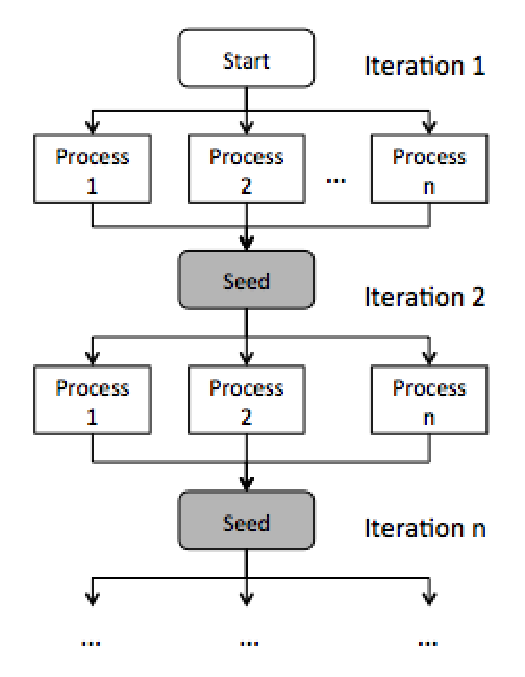
\includegraphics[width=2.9in,height=3.9in]{iterative_sampling}
  \caption{Iterative sampling procedures}
\label{iterative_sampling}
\end{figure}

Motivated by the previous work, we use multiple random restarts and iterative sampling process to improve decipherment \cite{Dou:2012}. As shown in Figure. The idea is to start a few sampling processes each with a different random sample. Then combine the results from different runs and use the combined results to initiate the next sampling iteration. The details of the sampling procedure are listed below:

 \begin{itemize}
  \item Extract dependency bigrams from parsing outputs and collect their counts.
  \item Keep bigrams whose counts are greater than a threshold $t$. Then start N different randomly seeded and initialized sampling processes. Perform sampling.
  \item At the end of sampling, extract word translation pairs $(f,e)$ from the final sample. Estimate translation probabilities $P(e|f)$  for each pair. Then construct a translation table by keeping translation pairs $(f,e)$ seen in more than one decipherment and use the average $P(e|f)$ as the new translation probability.
  \item Lower the threshold $t$ to include more bigrams into the sampling process. Start N different sampling processes again and initialize the first sample using the translation pairs obtained from the previous step (for each dependency bigram $f_{1},f_{2}$, find an English sequence $e_{1},e_{2}$, whose $P(e_{1}|f_{1})\cdot P(e_{2}|f_{2})\cdot P(e_{1},e_{2})$is the highest). Perform sampling again.
  \item Repeat until $t=1$.
\end{itemize}

In our Spanish-English decipherment experiments, we use 10 different random restarts. In experiments, we also gradually increase the weight of base distribution as more and more ciphtertext becomes available. We set the weight to 2, 10, and 50 for ciphertext with 100k, 1 million, and 10 million tokens respectively. 

\subsection{Evaluation Metrics}
We use type accuracy as our evaluation metric: Given a word type $f$ in Spanish, we find top 5 translation pairs $(f,e)$ ranked by $P(e|f)$ from the translation table learned through decipherment. If the translation pair $(f,e)$ can also be found in a gold translation lexicon $T_{gold}$, we treat the word type $f$ as correctly deciphered. Let $|C|$ be the number of word types correctly deciphered, and $|V|$ be the total number of word types evaluated. We define type accuracy as $\frac{|C|}{|V|}$.

To create $T_{gold}$, we use GIZA to align a small amount of Spanish-English parallel text (1 million tokens for each language), and use the lexicon derived from the alignment as our gold translation lexicon. $T_{gold}$ contains a subset of 4233 word types in the top 5000 frequent word types, and 7479 word types in the top 10k frequent word types. We decipher top 10k frequent Spanish word types to top 10k frequent English word types, and evaluate decipherment accuracy on both top 5k most frequent word types and all the 10k word types.

\section{Deciphering Malagasy}
\label{decipher_malagasy}
In this section, we first introduce the Malagasy language, and describe the data used in the experiments; then explain what makes deciphering Malagasy more challenging compared with Spanish, and differences in experiment settings for achieving higher decipherment accuracy.

\subsection{The Malagasy Language}
Malagasy is the official language of Madagascar. It has around 18 million native speakers. Although Madagascar is an African country, Malagasy belongs to the Malayo-Polynesian branch of the Austronesian language family. Malagasy and English have very different word orders. First of all, in contrast to English, which has a subject-verb-object (SVO) word order, Malagasy has a verb-object-subject (VOS) word order. Besides that, Malagasy is a typical head initial language: Determiners precede nouns, while other modifiers and relative clauses follow nouns (e.g. ny ``the'' boky ``book'' mena ``red''). The significant differences in word order pose great challenges for decipherment.


\subsection{Data}
We list the size of both monolingual and parallel data used in this experiment in Table \ref{mlg-en-data}. The data used in this experiment is released from previous work by \newcite{dou-vaswani-knight:2014:EMNLP2014}. The monolingual data in Malagasy contains news data collected from various local websites. The English monolingual data contains Gigaword and additional 300 million tokens of news on Africa. The parallel data is collected from GlobalVoices, a multilingual news website, where volunteers translate news into different languages. The parallel data is used to build a dictionary for evaluating decipherment accuracy. 

 \begin{table}
 \begin{center}
 \begin{tabular}{ |c|c|c| } \hline
             & Malagasy & English \\ \hline
\multirow{2}{*}{Non Parallel} & 16 million & 1.2 billion\\ 
& (Web) & \pbox{2cm}{ (Gigaword \\ and Web)}  \\ \hline
\multirow{2}{*}{Parallel} & 2.0 million& 1.8 million \\
 & (GlobalVoices) & (GlobalVoices)  \\ \hline
 \end{tabular}
 \caption{Size of data in tokens used in Malagasy-English decipherment}
 \label{mlg-en-data}
 \end{center}
 \end{table}
 
\subsection{Systems}
The baseline system is the same as the baseline used in Spanish-English decipherment experiments. We use data provided in previous work \cite{dou-vaswani-knight:2014:EMNLP2014} to build a Malagasy dependency parser. For English, we use Turbo parser trained on Penn Treebank \cite{TurboParser}.  

Since the Malagasy parser doesn't predict dependency relation types, we use head-child part-of-speech (POS) tag patterns to select a subset of dependency bigrams for decipherment. We list the selected POS tag patterns in Table \ref{mlg-en-dep-type}.

%
 \begin{table}
 \begin{center}
 \begin{tabular}{ |c|c| } \hline
          Head POS & Child POS \\ \hline
Verb & Noun \\ \hline
Verb & Proper Noun \\ \hline
Verb & Person Pronoun \\ \hline
Preposition & Noun \\ \hline
Preposition & Proper Noun \\ \hline
Noun & Adjective \\ \hline
Noun & Determiner \\ \hline
Noun & Verb Particle \\ \hline
Noun & Verb Noun \\ \hline
Noun & Cardinal Number \\ \hline
Noun & Noun \\ \hline
 \end{tabular}
 \caption{Head-Child POS patterns used in decipherment}
 \label{mlg-en-dep-type}
 \end{center}
 \end{table}
%

\subsection{Sampling Procedure}
We use the same sampling protocol designed for Spanish-English decipherment. However, in experiments, we find out that simply using viterbi decoding to initialize the first sample does not work as well as in deciphering Spanish. Therefore, in addition to using Viterbi decoding, we also initialize the base distribution to the base distribution of previous decipherment that produces highest decipherment accuracy.

Compared with Spanish-English decipherment, we find the base distribution plays a more important role in achieving higher decipherment accuracy for Malagasy-English. Therefore, we set weight to 10, 100, and 500 when deciphering 100k, 1 million, and 20 million ciphtertext respectively.


%
 \begin{table*}[!ht]
 \begin{center}
 \begin{tabular}{ |c|c|c|c|c|c|c|c|c| } \hline
         & \multicolumn{4}{|c|}{Spanish-English} & \multicolumn{4}{|c|}{Malagasy-English} \\ \hline
 Top &  \multicolumn{2}{|c|}{5k} & \multicolumn{2}{|c|}{10k} & \multicolumn{2}{|c|}{5k} & \multicolumn{2}{|c|}{10k} \\ \hline
 System &  Baseline & DMRE & Baseline & DMRE &  Baseline & DMRE & Baseline & DMRE \\ \hline
 100k &  1.9 & 12.4 & 1.1 & 7.1 &  1.2 & 2.7 & 0.6 & 1.4 \\ \hline
 1 million &  7.3 & 37.7& 4.2 & 23.6 &  2.5 & 5.8 & 1.3 & 3.2 \\ \hline
 10 million &  26.0 & 59.0 & 15.9 & 43.7 &  5.4 & (12.1) & 3.0 & (7.2) \\ \hline
 \end{tabular}
 \caption{Spanish-English and Malagasy-English decipherment accuracy (\%) of top 5k and 10k most frequent word types}
 \label{decipher-acc-result}
 \end{center}
 \end{table*}
%

\subsection{Results}
In experiments, we gradually increase the size of ciphertext and compare decipherment accuracy of baseline with our new approach. We evaluate accuracy for top 5k and 10k most frequent word types for each language pair, and present them in Table \ref{decipher-acc-result}; 


 \begin{figure}[!ht]
  \centering
  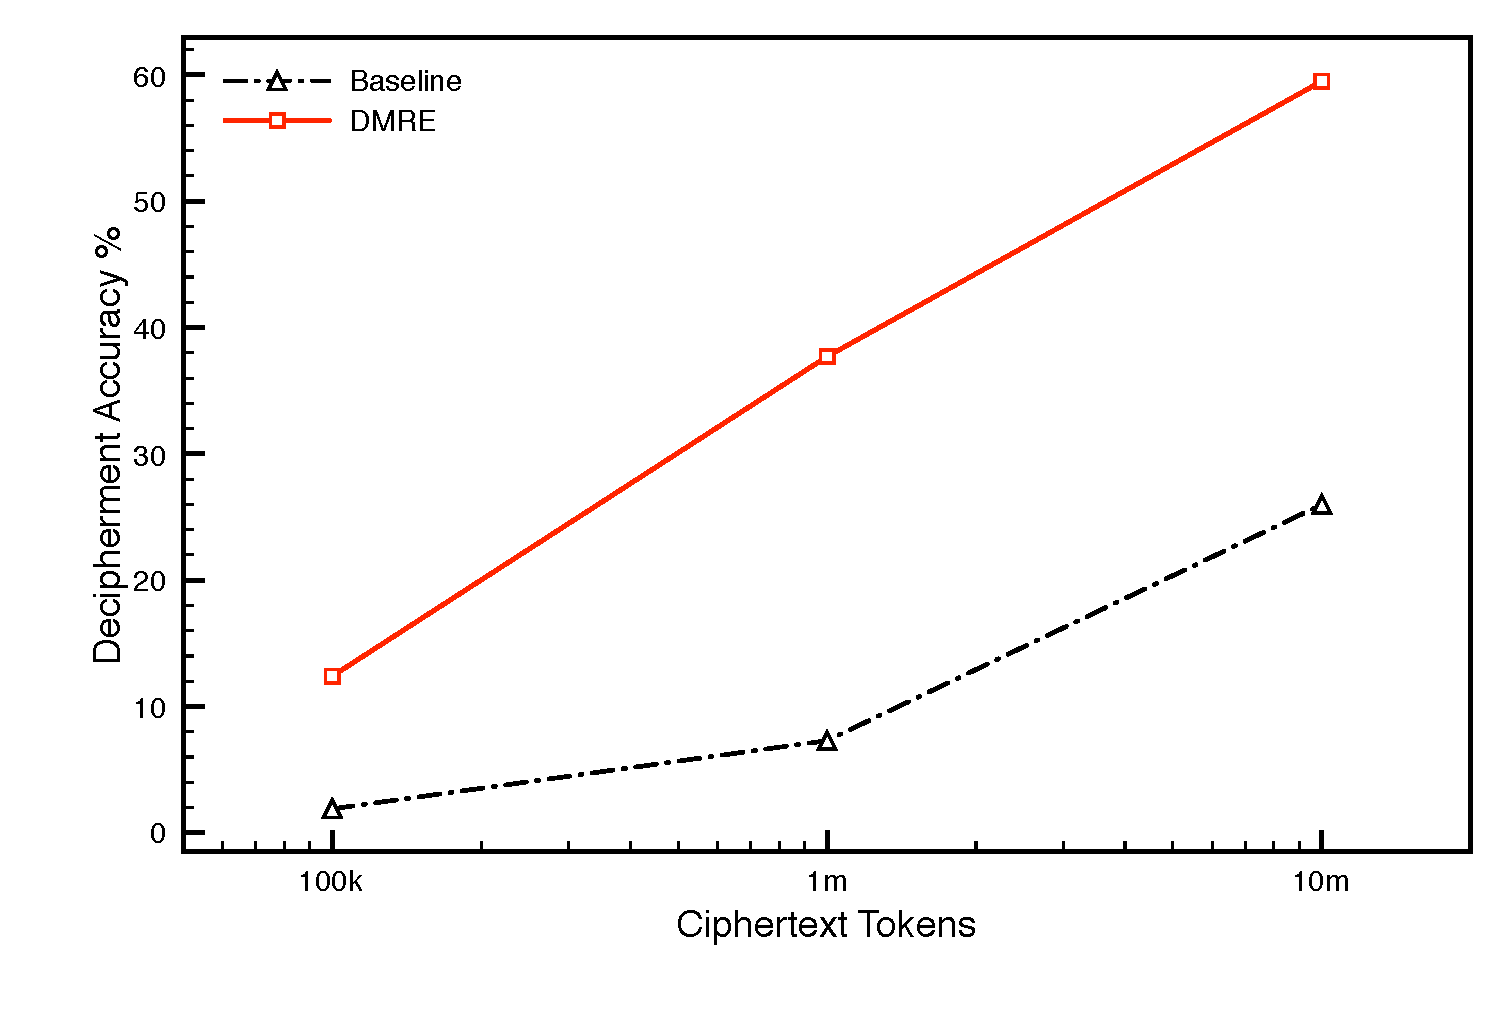
\includegraphics[width=3.1in,height=2.4in]{es_en_curve}
  \caption{Learning curves for Spanish-English decipherment.}
\label{es-en-curve}
\end{figure}

To better visualize the improvement, we also present the learning curves of decipherment accuracy for top 5k most frequent word types. Figure \ref{es-en-curve} compares baseline with our new approach in deciphering Spanish into English. With 100k tokens of Spanish text, the baseline achieves 1.9\% accuracy, while the new system achieves 12.4\% accuracy, which improves the baseline by over 6 times. The improvement holds consistently throughout the experiment. In the end, the baseline achieves 22\% accuracy, while the new system achieves 60\% accuracy, nearly 3 folds higher. 

 \begin{figure}[!ht]
  \centering
  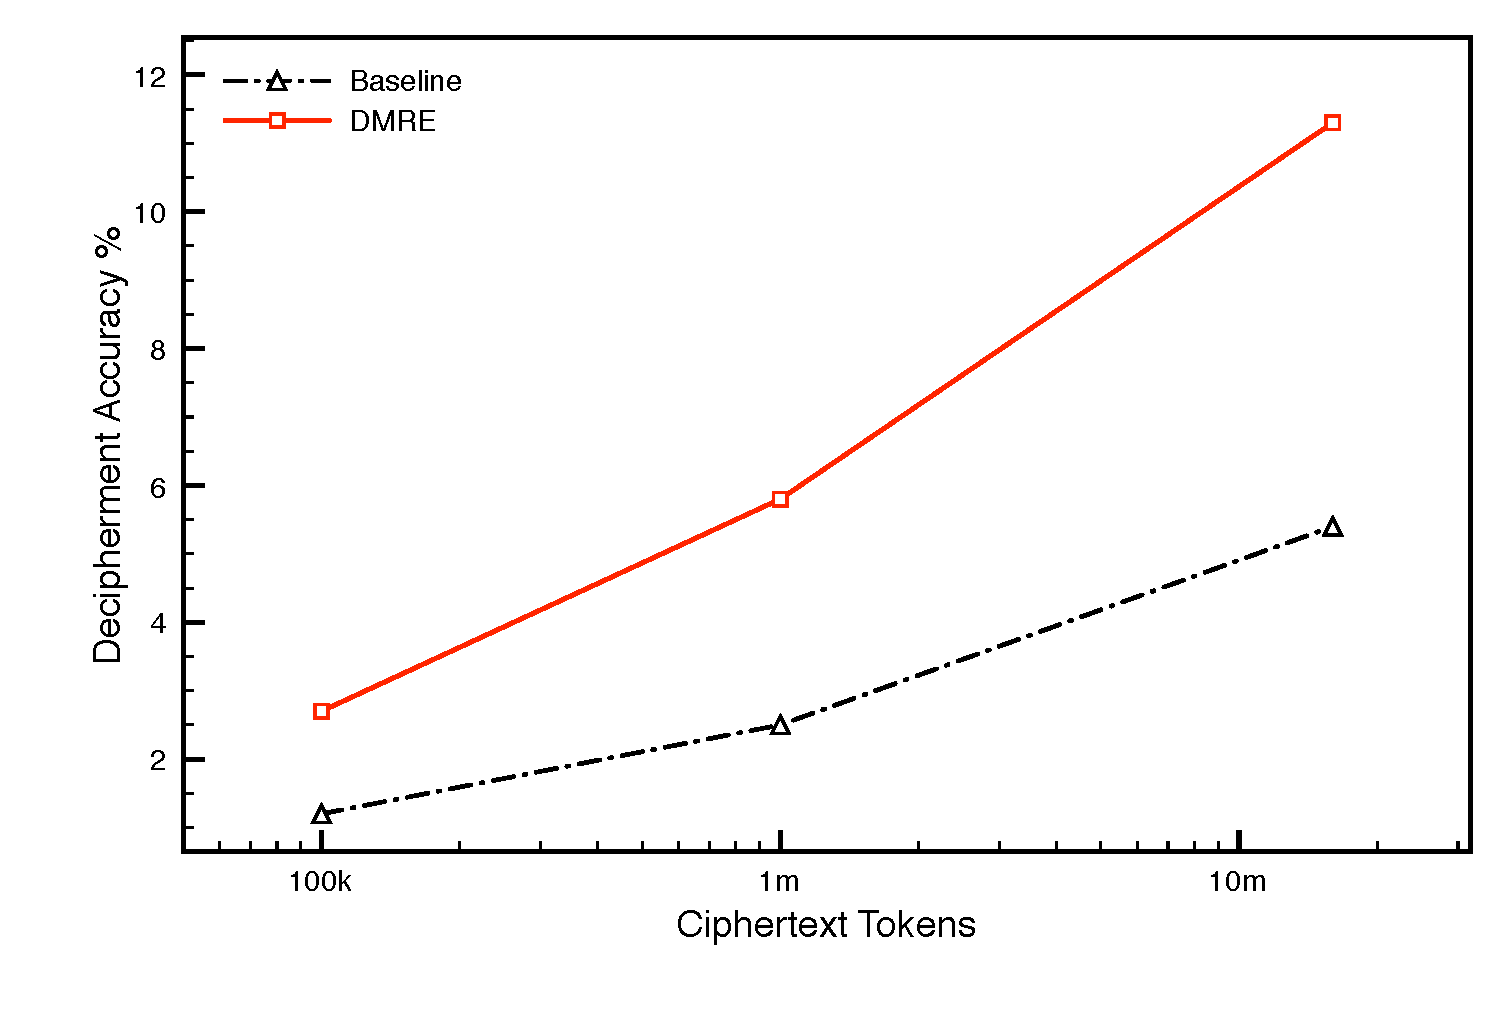
\includegraphics[width=3.1in,height=2.4in]{mlg_en_curve}
  \caption{Learning curves for Malagasy-English decipherment.}
\label{mlg-en-curve}
\end{figure}


Figure \ref{mlg-en-curve} compares baseline with our new approach in deciphering Malagasy into English. With 100k tokens of data, the baseline achieves 1.2\% accuracy, while the new system achieves 2.4\% accuracy.  We observe consistent improvement throughout the experiment. In the end, the baseline accuracy climbs to 5.8\%, while the new system improves it to 12.0\%.

Overall, the improvement we achieved is solid, and is observed across different language pairs. When we exam the base distribution, we find that the correct translations have higher probability. This helps prevent the language model driving deicpherment to a wrong direction. 

 






\section{Conclusion and Future Work}
We propose a new framework that simultaneously performs decipherment and learns mapping of word embeddings. The mapping is then used to give decipherment a better base distribution. Experiment results show that our new algorithm improves the state-of-the-art decipherment accuracy significantly: from 22\% to 60\% for Spanish-English, and 5.8\% to 12.0\% for Malagasy-English. The improvement could lead to further advances in using monolingual data for better quality MT
In the future, we will work on making the new method scale to much larger vocabulary size, and apply it to improve MT systems.
\section*{Acknowledgments}
%This work was supported by NSF Grant 0904684 and ARO grant W911NF-10-1-0533. The authors would like to thank David Chiang, Malte Nuhn, Victoria Fossum, Ashish Vaswani, Ulf Hermjakob, Yang Gao, and Hui Zhang (in no particular order) for their comments and suggestions.




\bibliography{ref}
\bibliographystyle{acl}

\end{document} 